
\section{Ergebnis des zweiten Ideationszyklus mit der Lotus-Blossom-Methode} \label{appendix:lotus_blossom}

\begin{figure}[H]
  \centering
  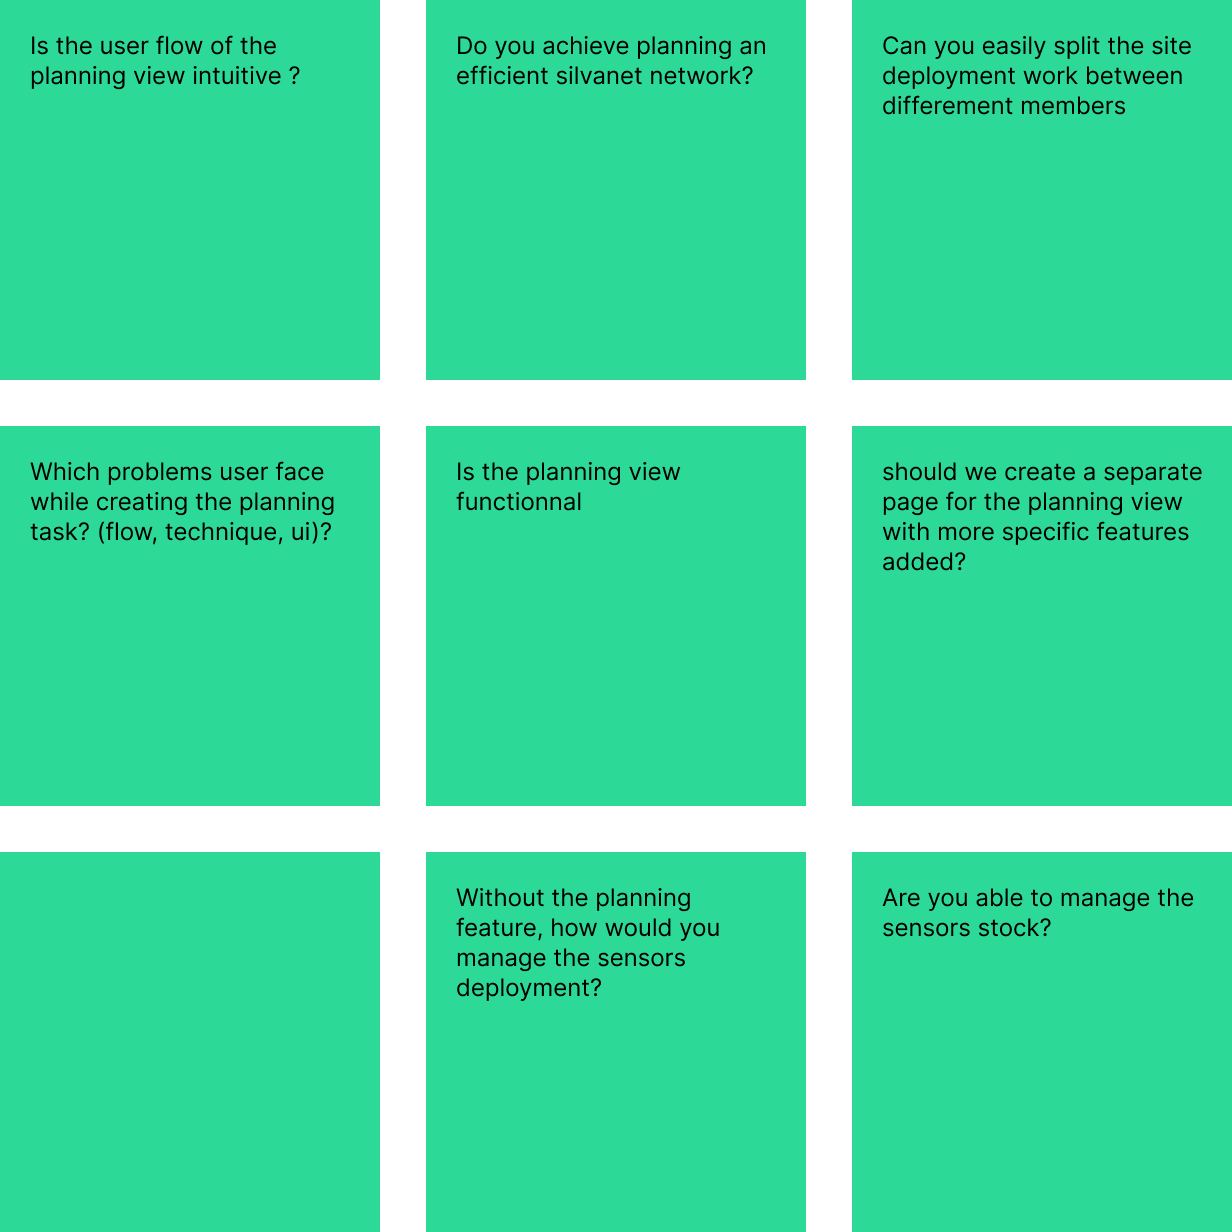
\includegraphics[width=10cm]{lotus_blossom_top}
  \caption{}
  \label{fig:lotus_blossom_top}
\end{figure}
\begin{figure}[H]
  \centering
  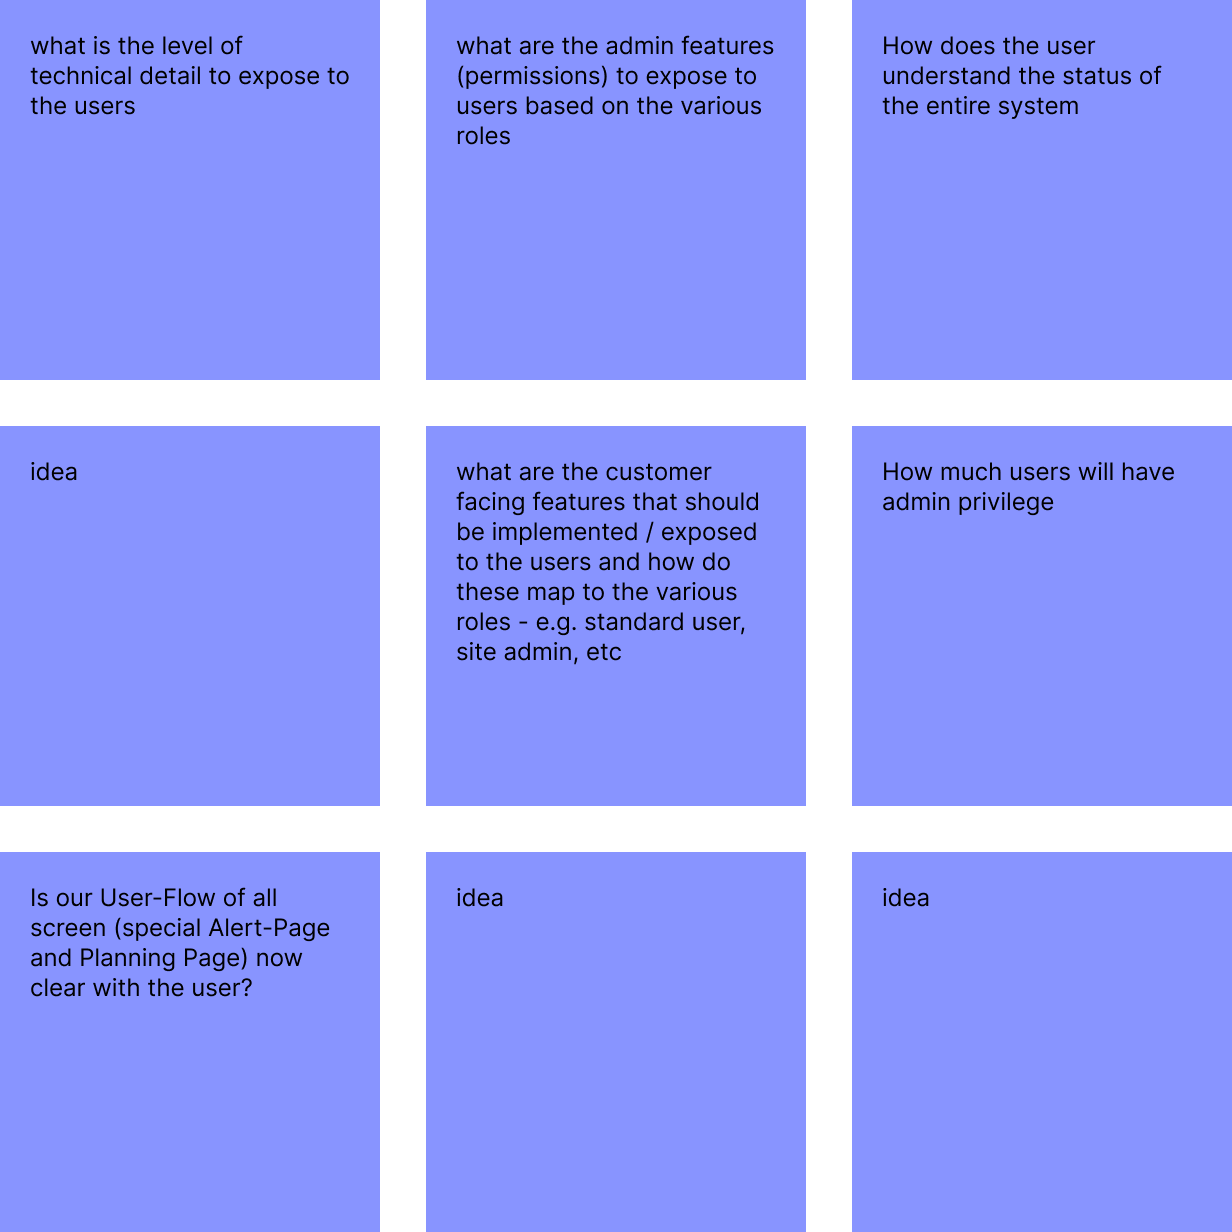
\includegraphics[width=10cm]{lotus_blossom_right}
  \caption{}
  \label{fig:lotus_blossom_right}
\end{figure}
\begin{figure}[H]
  \centering
  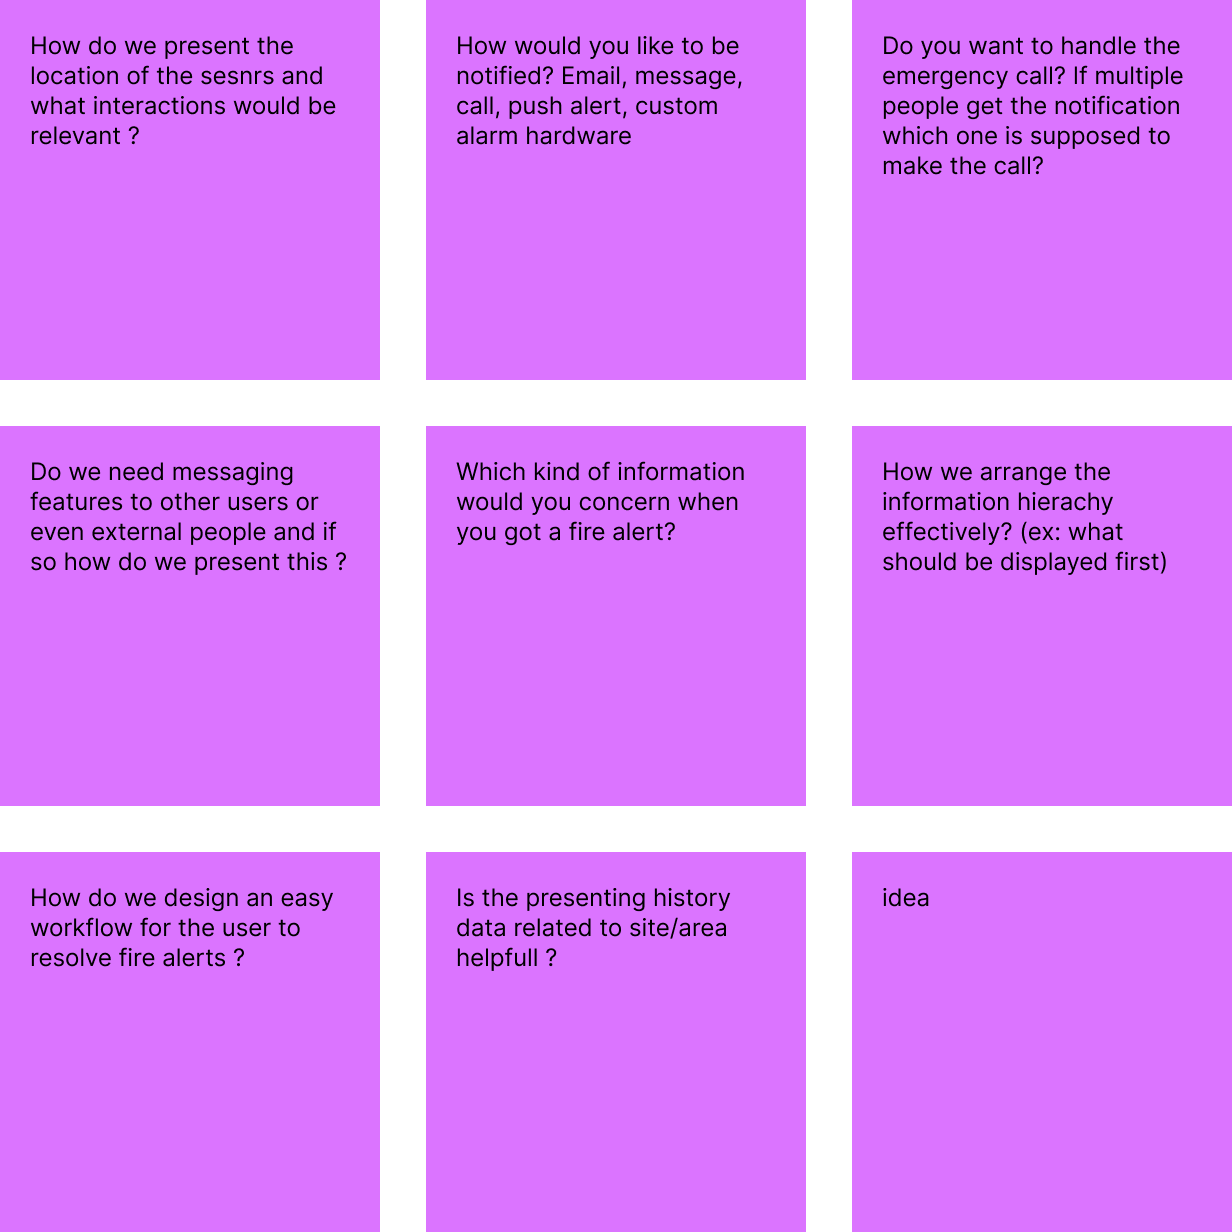
\includegraphics[width=10cm]{lotus_blossom_bottom_right}
  \caption{}
  \label{fig:lotus_blossom_bottom_right}
\end{figure}
\begin{figure}[H]
  \centering
  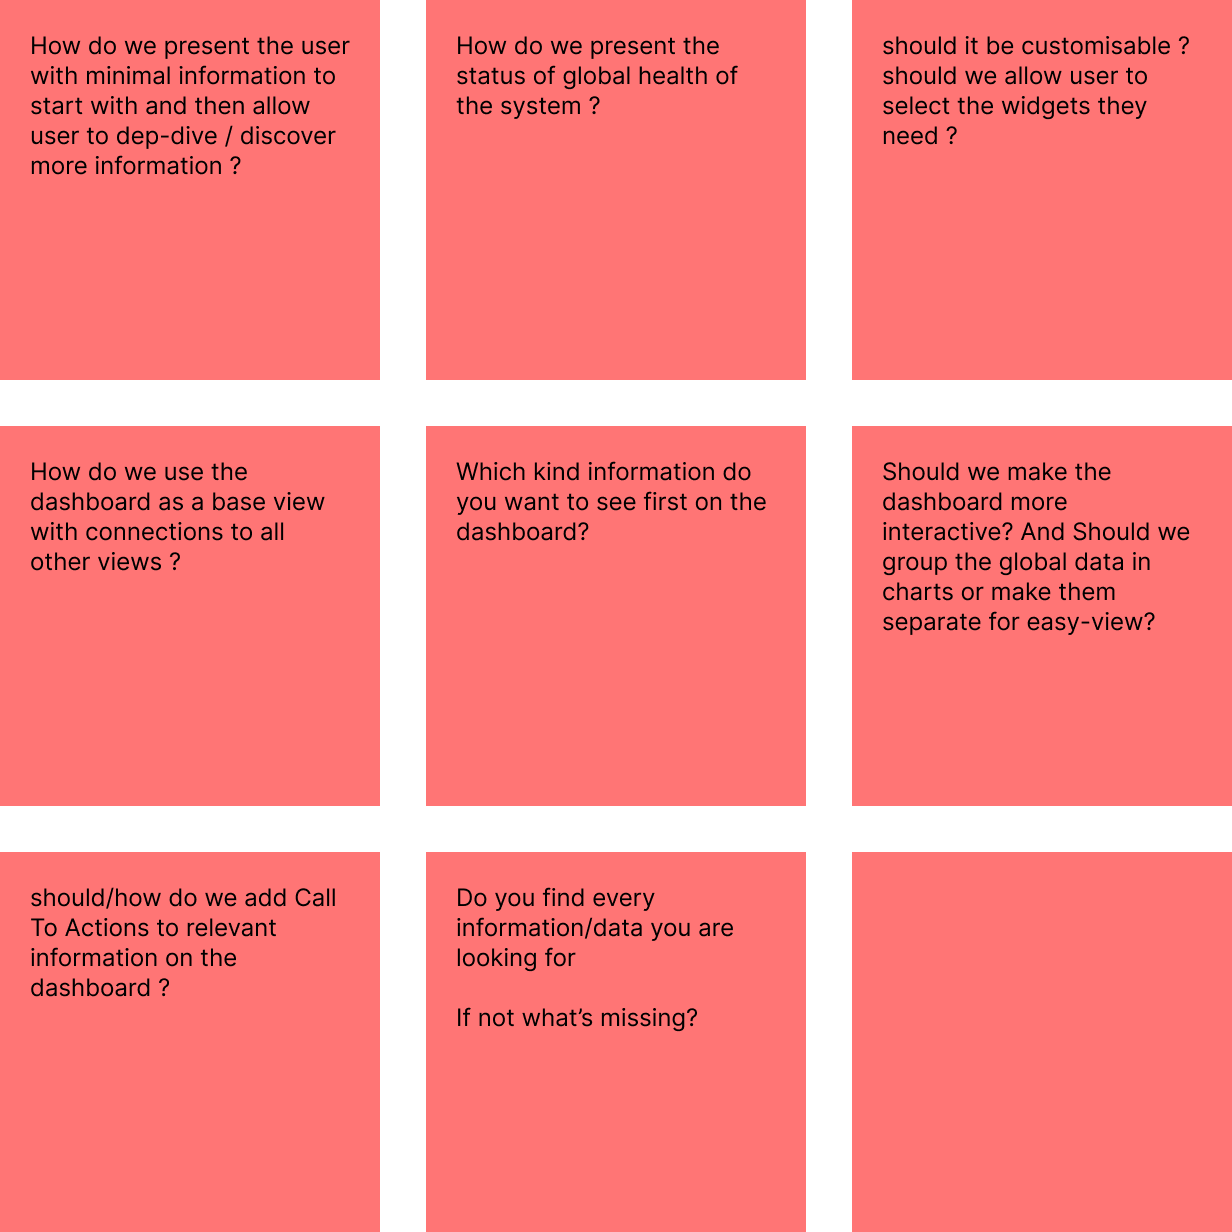
\includegraphics[width=10cm]{lotus_blossom_bottom}
  \caption{}
  \label{fig:lotus_blossom_bottom}
\end{figure}
\begin{figure}[H]
  \centering
  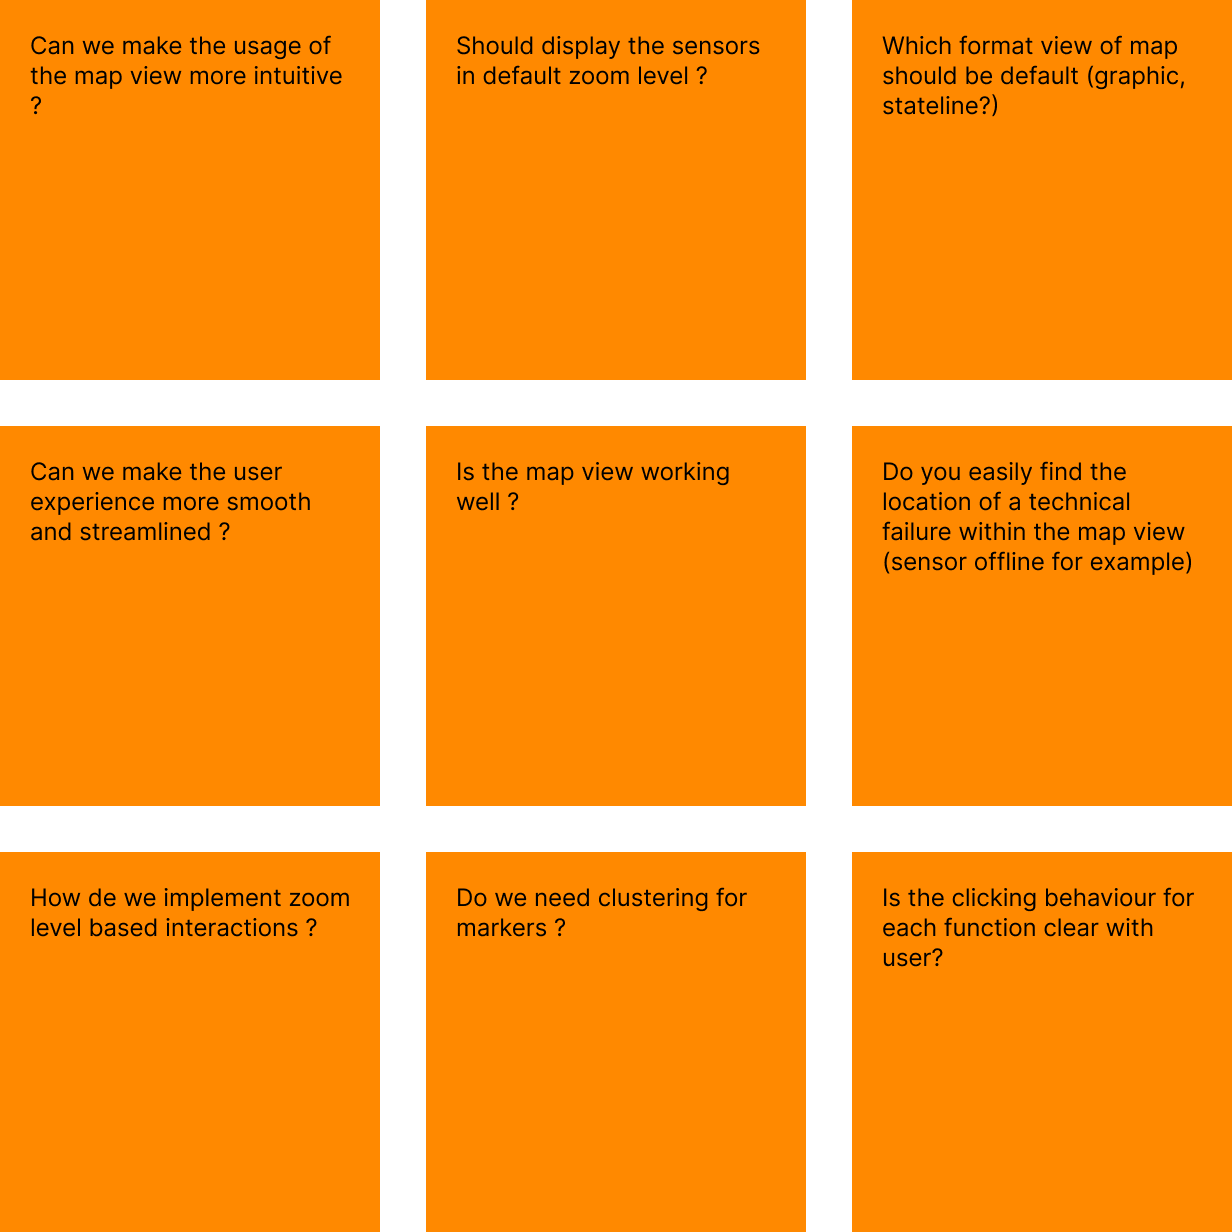
\includegraphics[width=10cm]{lotus_blossom_bottom_left}
  \caption{}
  \label{fig:lotus_blossom_bottom_left}
\end{figure}
\begin{figure}[H]
  \centering
  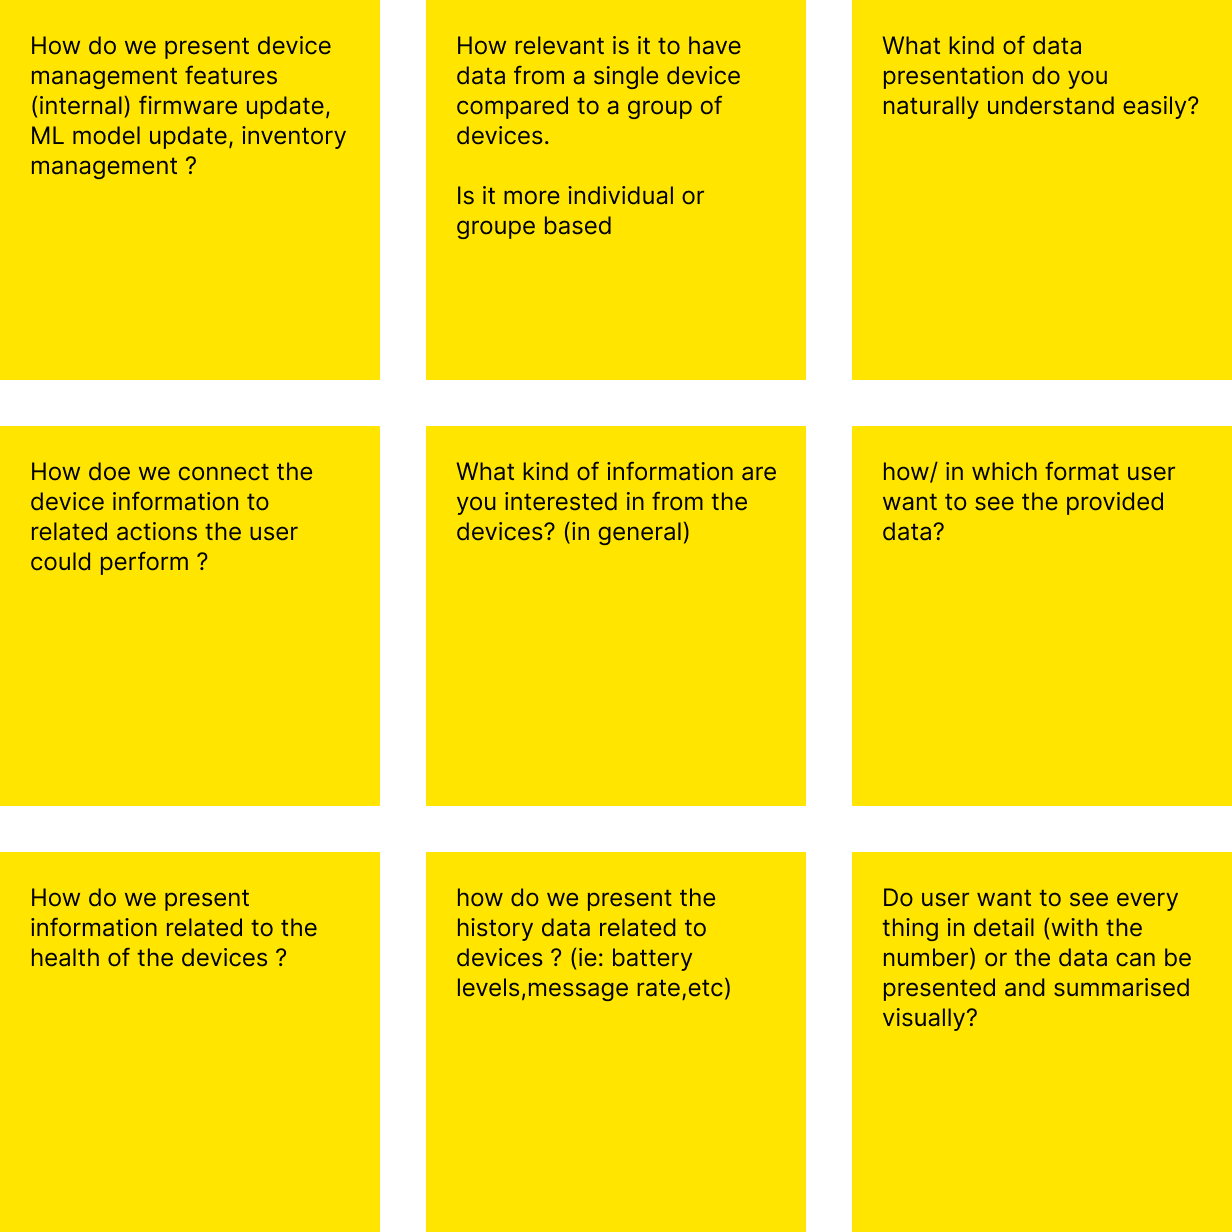
\includegraphics[width=10cm]{lotus_blossom_top_left}
  \caption{}
  \label{fig:lotus_blossom_top_left}
\end{figure}

\section{Ergebnis der UX-Methode des Question Board, das von Dryads Cloud-Team mit dem Miro-Tool erstellt wurde} \label{appendix:question_board}

\begin{figure}[H]
  \centering
  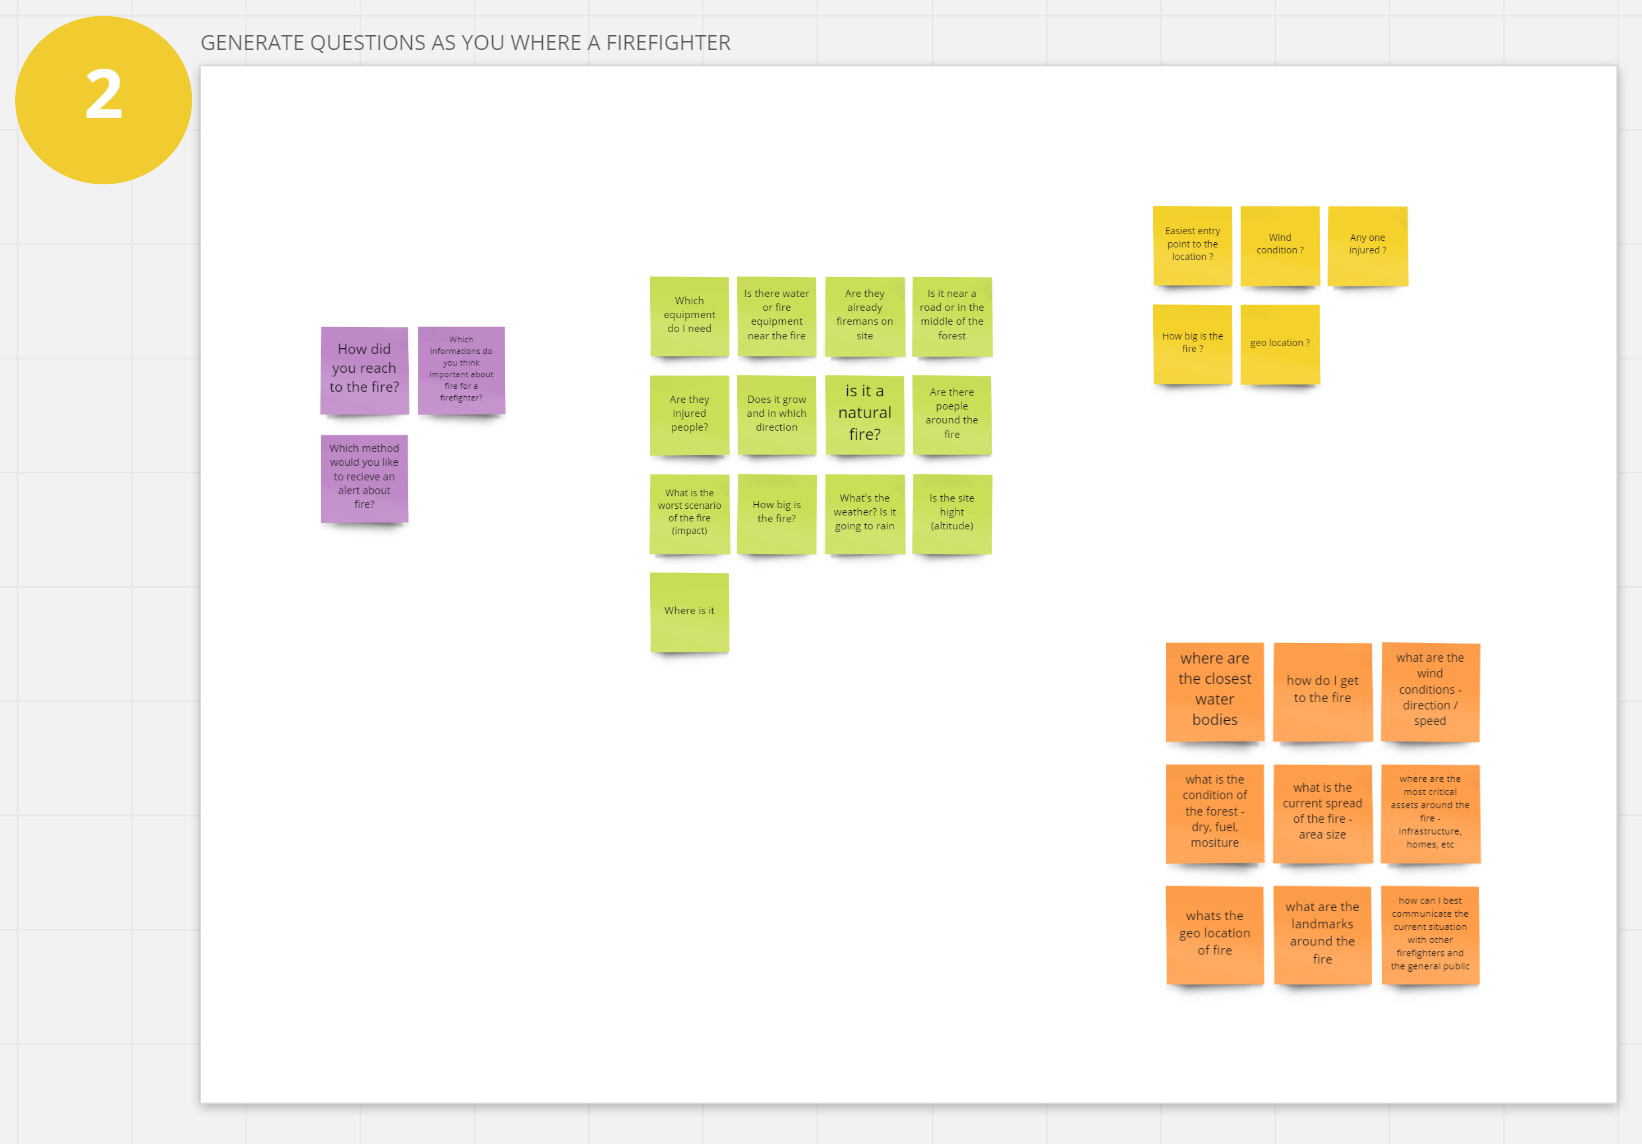
\includegraphics[width=\textwidth]{question_board_2}
  \caption{}
  \label{fig:question_board_2}
\end{figure}
\begin{figure}[H]
  \centering
  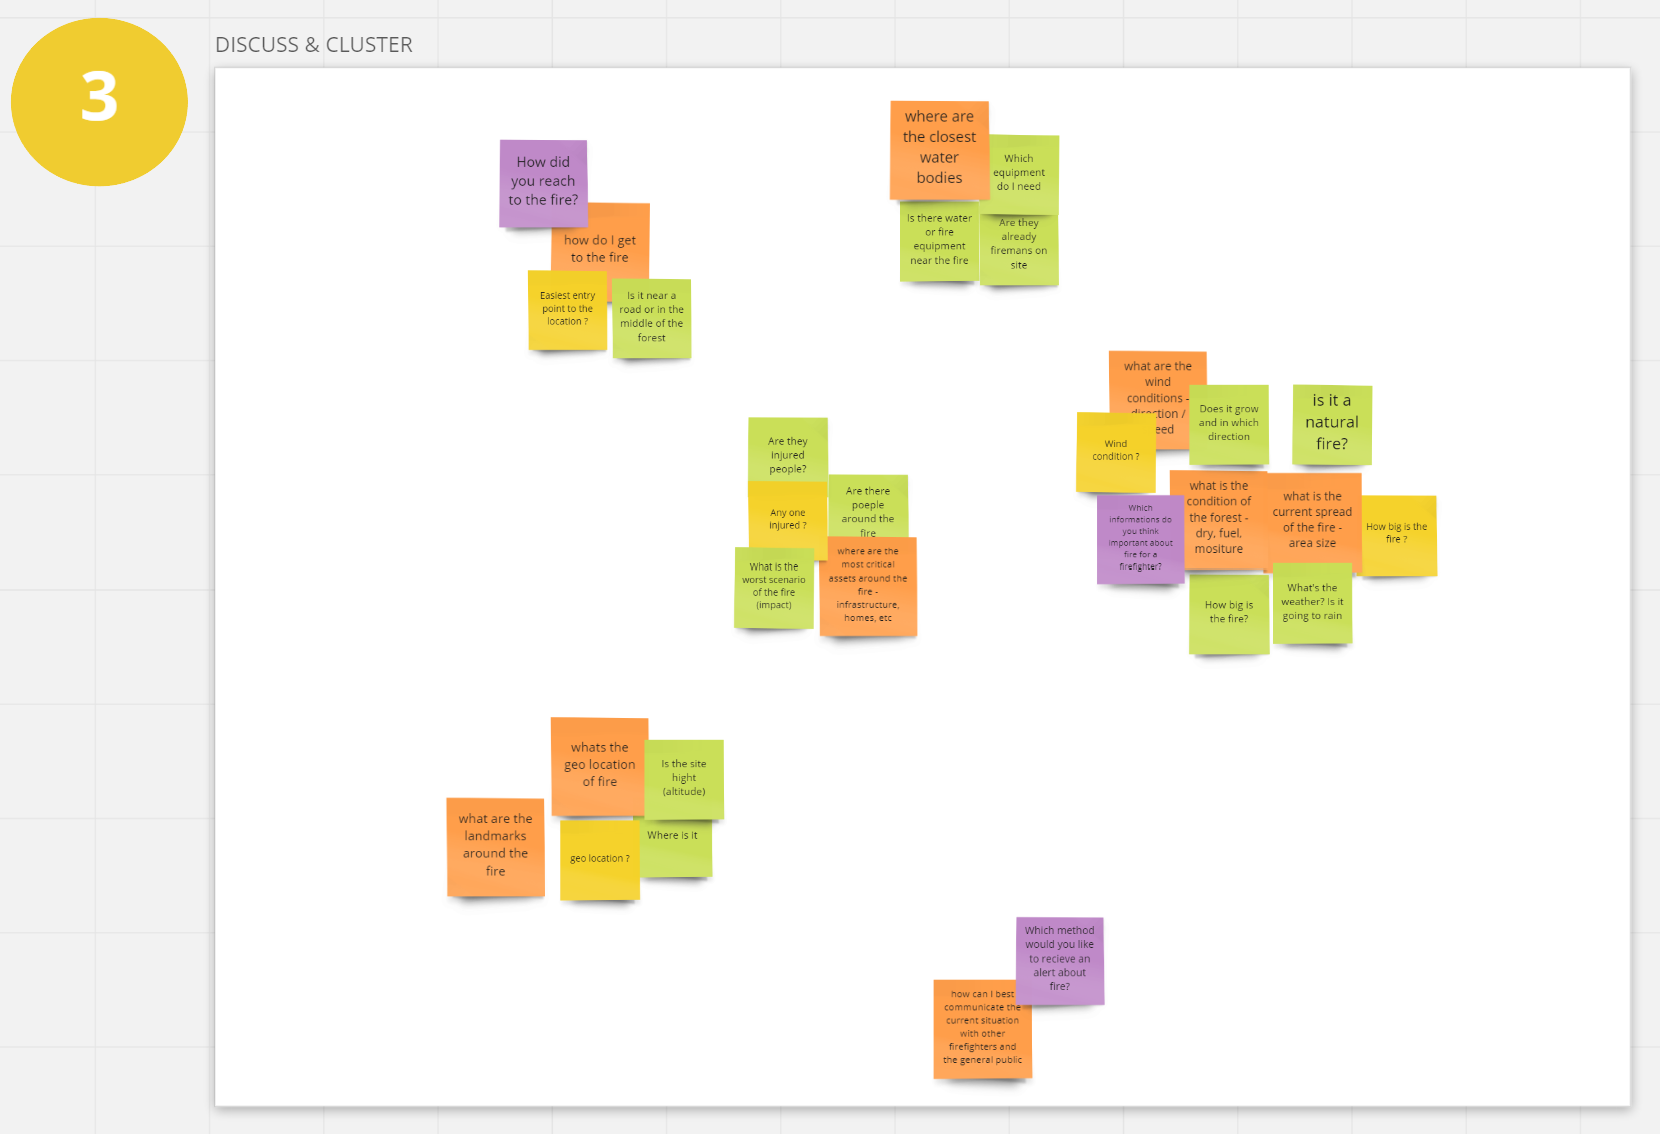
\includegraphics[width=\textwidth]{question_board_3}
  \caption{}
  \label{fig:question_board_3}
\end{figure}
\begin{figure}[H]
  \centering
  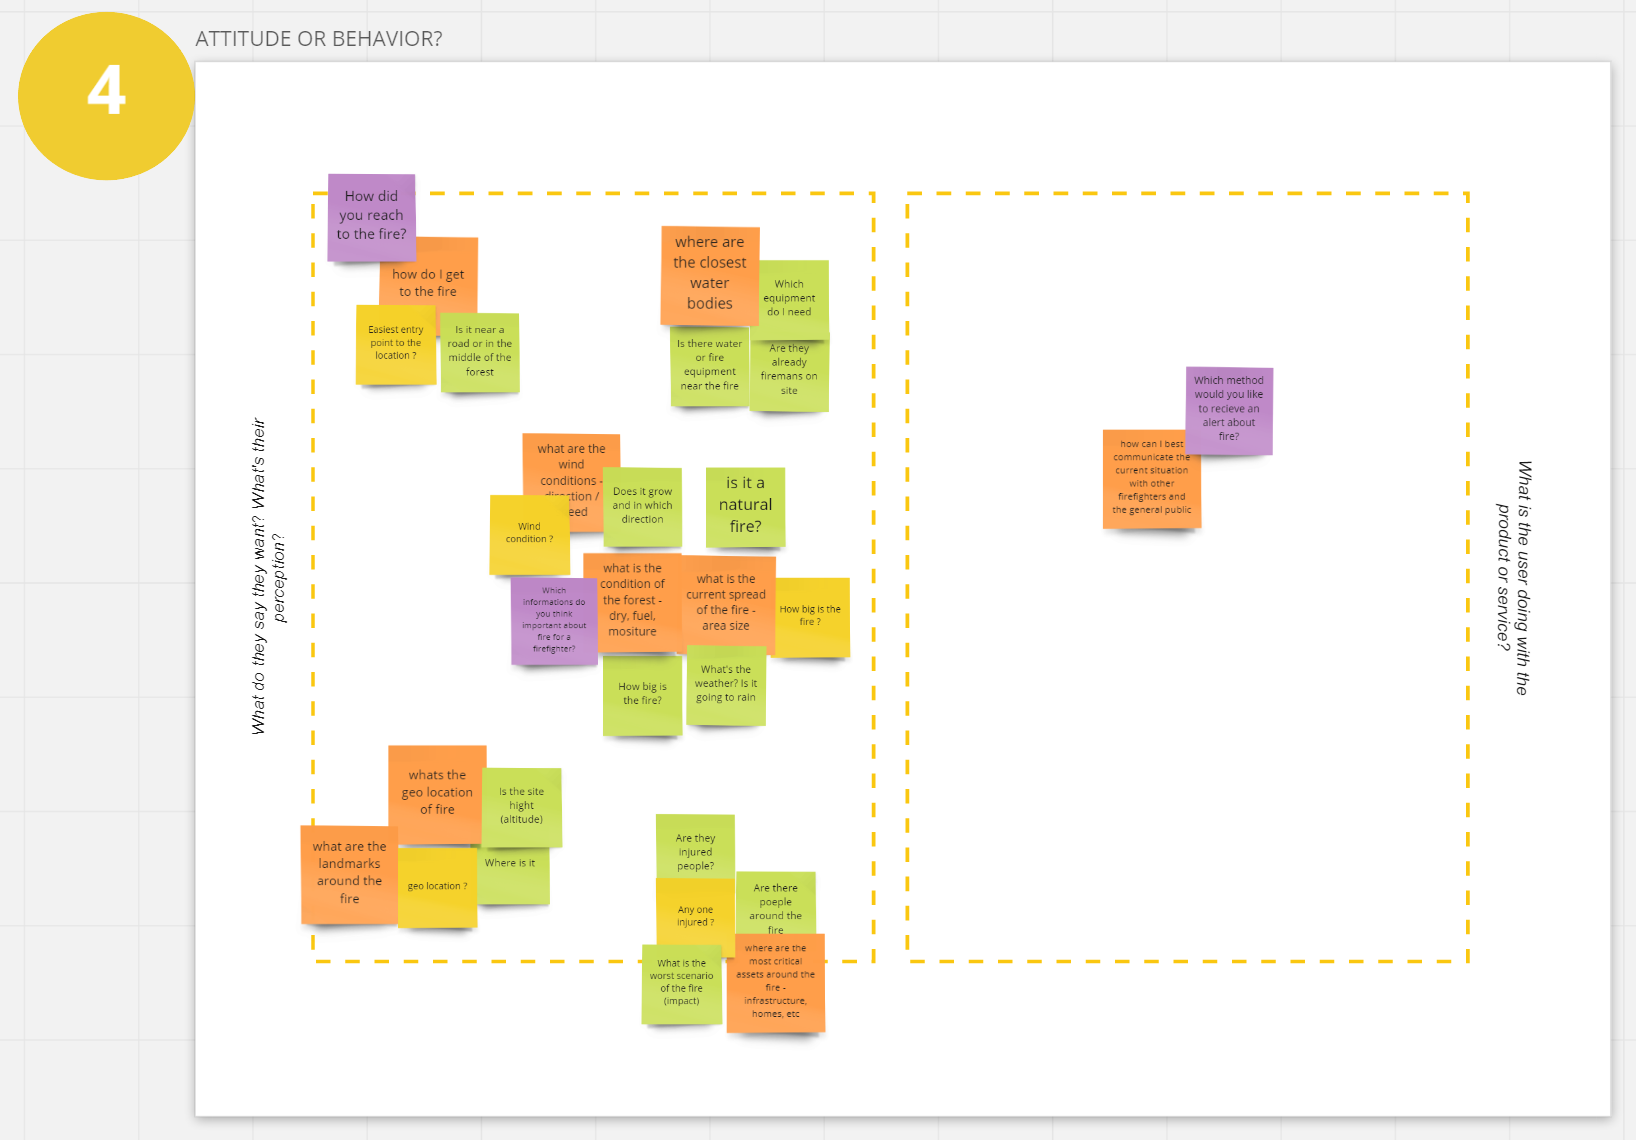
\includegraphics[width=\textwidth]{question_board_4}
  \caption{}
  \label{fig:question_board_4}
\end{figure}
\begin{figure}[H]
  \centering
  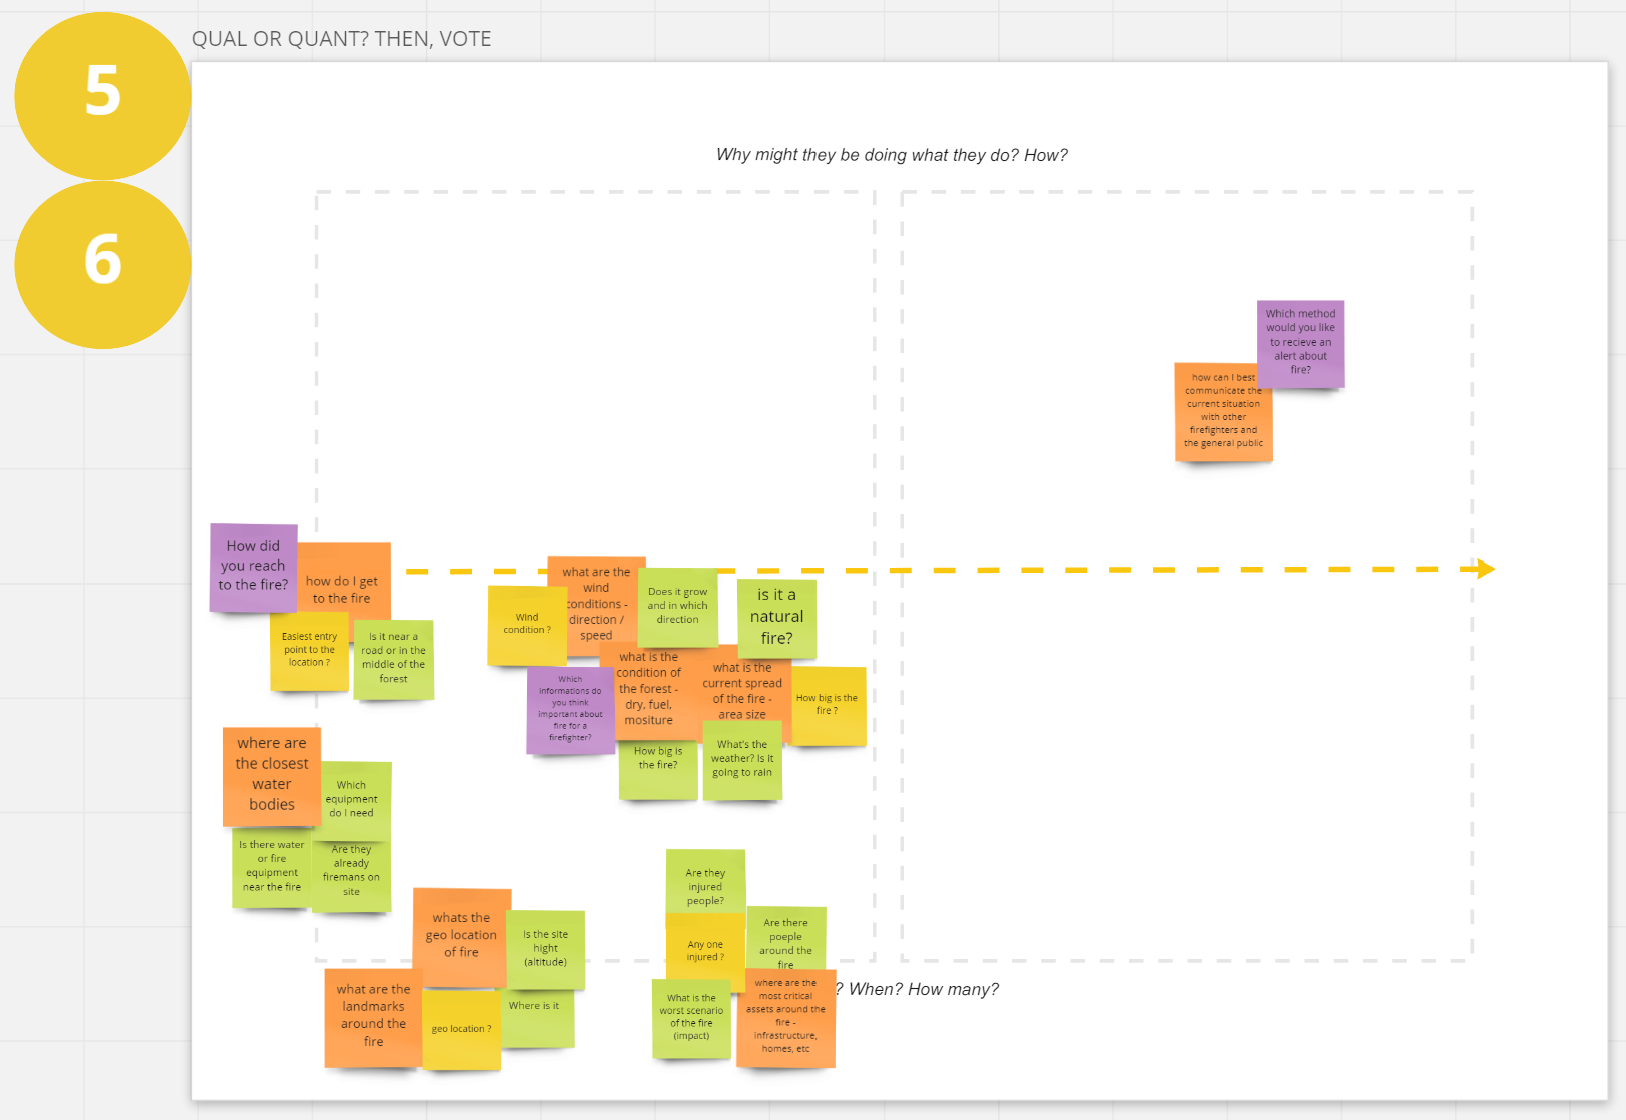
\includegraphics[width=\textwidth]{question_board_5}
  \caption{}
  \label{fig:question_board_5}
\end{figure}
\begin{figure}[H]
  \centering
  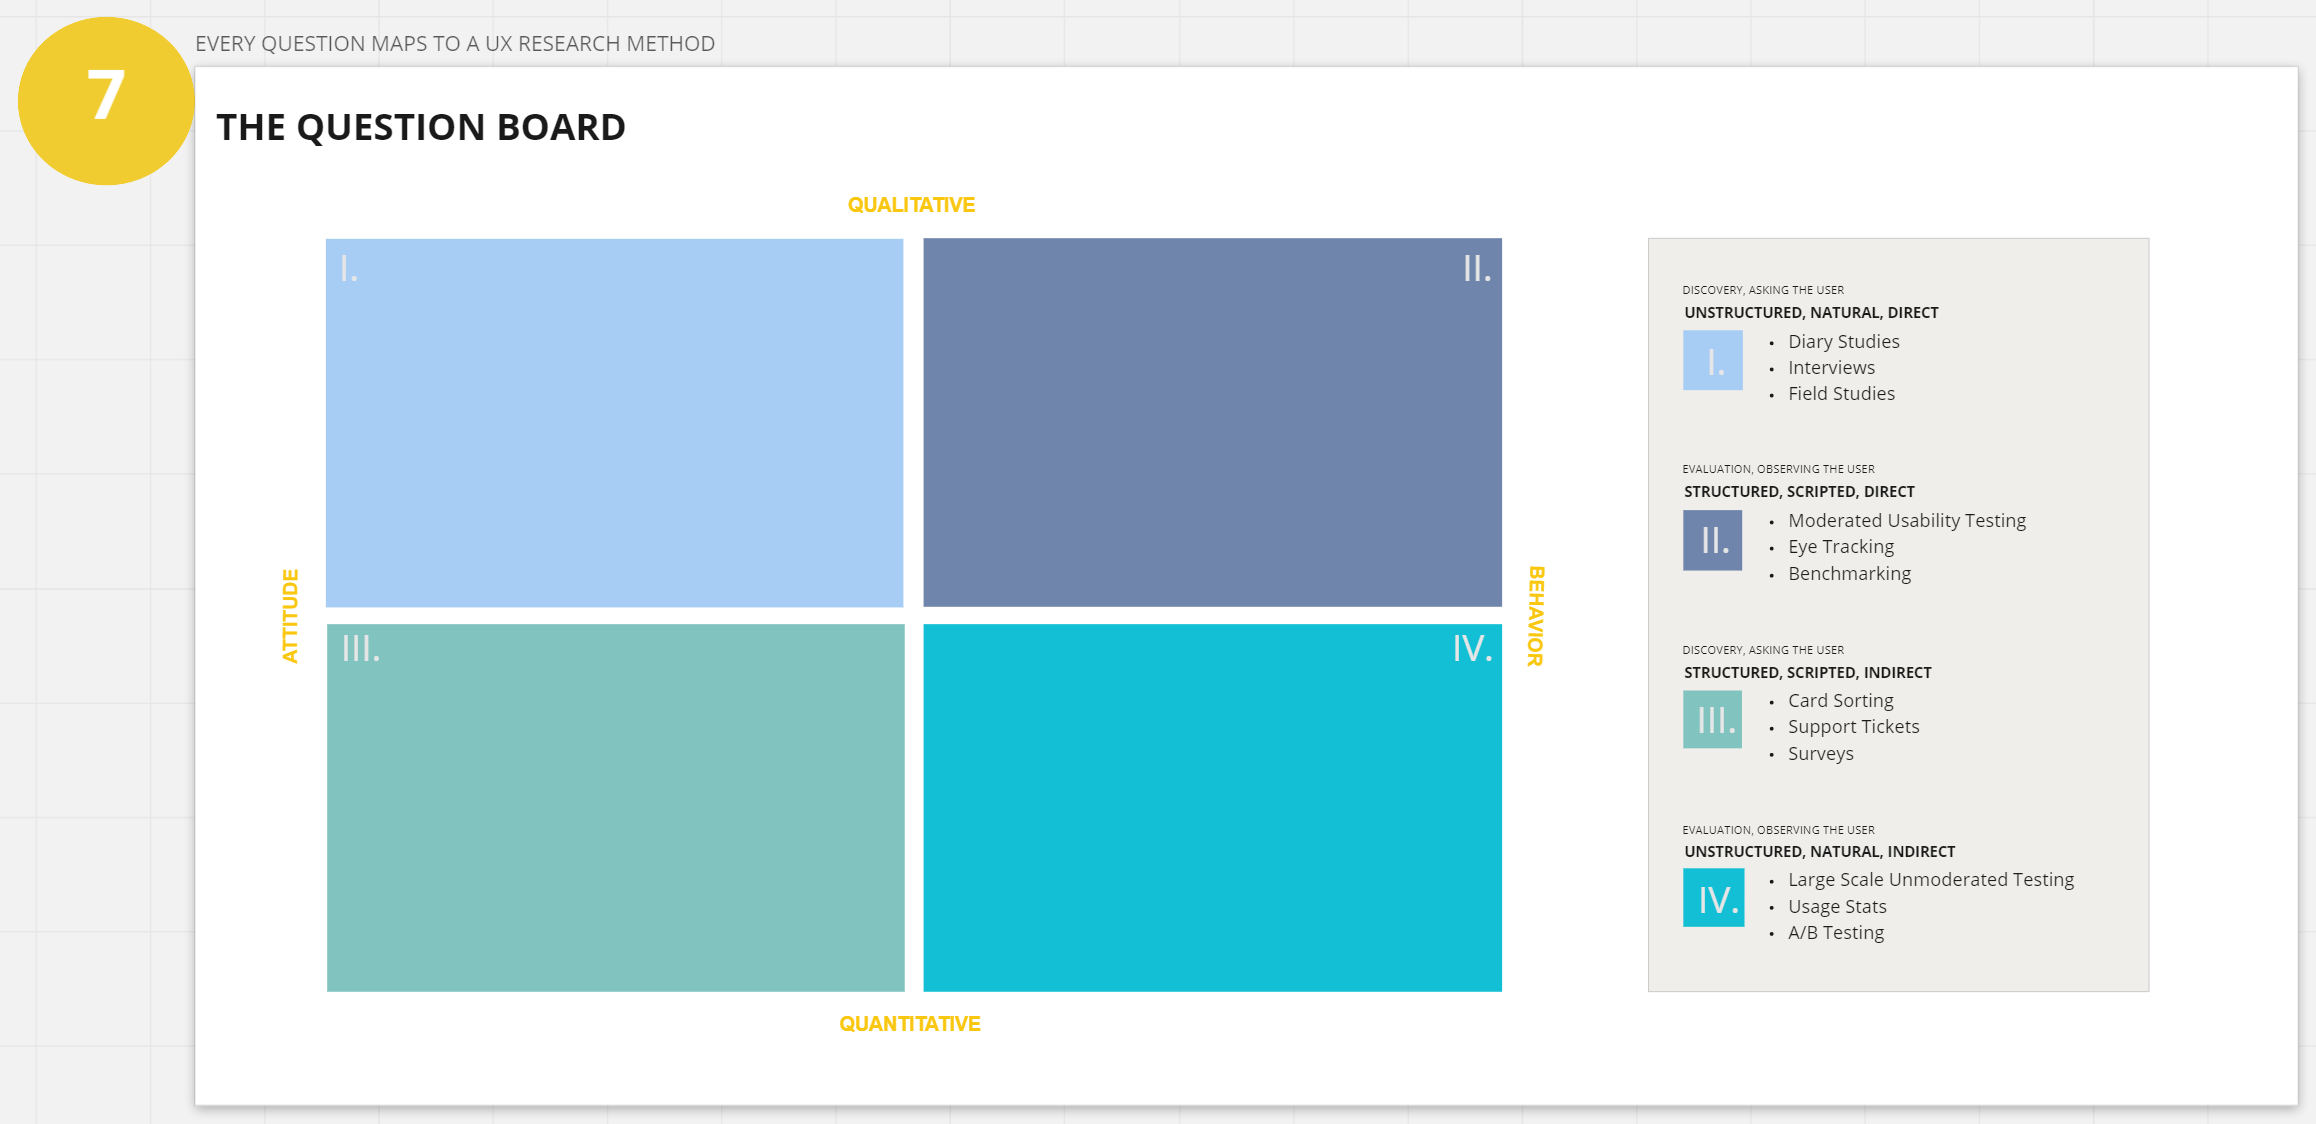
\includegraphics[width=\textwidth]{question_board_7}
  \caption{}
  \label{fig:question_board_7}
\end{figure}

\section{Notizen aus der ergonomischen Inspektion der Webschnittstelle (Englisch)}

\includepdf[
  pages=-,
  scale=0.75,
  pagecommand={\label{dryad-ergonomic-inspection}\thispagestyle{plain}}
]{Statics/dryad-ergonomic-inspection.pdf}

\section{Formular für die Gemeinschaft der Feuerwehrleute (Deutsch)} \label{appendix:firefighter-survey}

\includepdf[
  pages=-,
  scale=0.75,
  pagecommand={\label{firefighter-survey-overview}\thispagestyle{plain}}
]{Statics/firefighter-survey-overview.pdf}

